\documentclass[border=4pt]{standalone}

\usepackage{amsmath}
\usepackage{tikz}
\usepackage{mathdots}
\usepackage{yhmath}
\usepackage{cancel}
\usepackage{color}
\usepackage{siunitx}
\usepackage{array}
\usepackage{multirow}
\usepackage{amssymb}
\usepackage{gensymb}
\usepackage{tabularx}
\usepackage{booktabs}
\usetikzlibrary{fadings}
\usetikzlibrary{patterns}


\begin{document}
 




\tikzset{every picture/.style={line width=0.75pt}} %set default line width to 0.75pt        

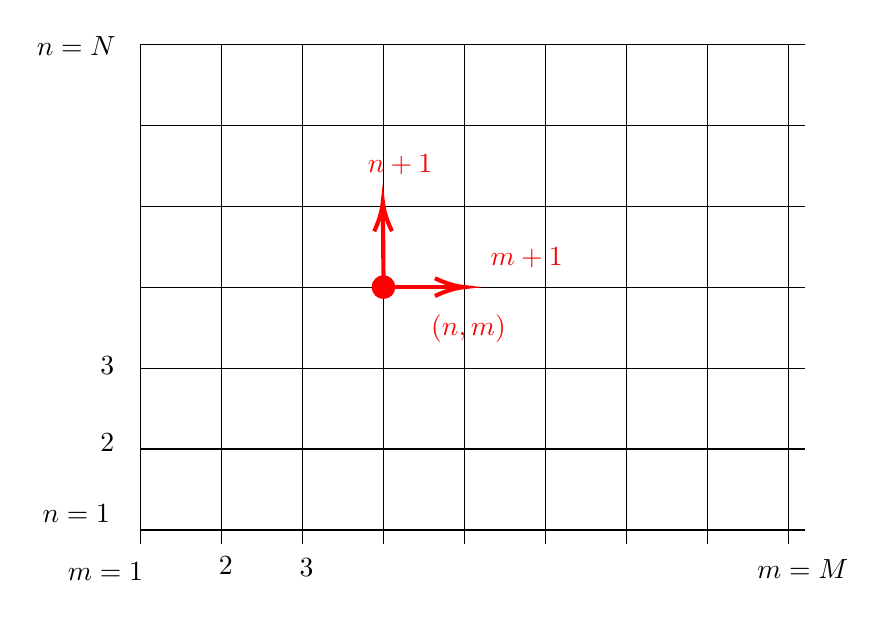
\begin{tikzpicture}[x=0.75pt,y=0.75pt,yscale=-1,xscale=1]
%uncomment if require: \path (0,300); %set diagram left start at 0, and has height of 300

%Shape: Grid [id:dp9112763349437901] 
\draw  [draw opacity=0] (80,28) -- (400,28) -- (400,269) -- (80,269) -- cycle ; \draw   (80,28) -- (80,269)(119,28) -- (119,269)(158,28) -- (158,269)(197,28) -- (197,269)(236,28) -- (236,269)(275,28) -- (275,269)(314,28) -- (314,269)(353,28) -- (353,269)(392,28) -- (392,269) ; \draw   (80,28) -- (400,28)(80,67) -- (400,67)(80,106) -- (400,106)(80,145) -- (400,145)(80,184) -- (400,184)(80,223) -- (400,223)(80,262) -- (400,262) ; \draw    ;
%Shape: Circle [id:dp3896605449828895] 
\draw  [color={rgb, 255:red, 255; green, 0; blue, 0 }  ,draw opacity=1 ][fill={rgb, 255:red, 255; green, 0; blue, 0 }  ,fill opacity=1 ] (191.57,145) .. controls (191.57,142) and (194,139.57) .. (197,139.57) .. controls (200,139.57) and (202.43,142) .. (202.43,145) .. controls (202.43,148) and (200,150.43) .. (197,150.43) .. controls (194,150.43) and (191.57,148) .. (191.57,145) -- cycle ;
%Straight Lines [id:da9636012117349724] 
\draw [color={rgb, 255:red, 255; green, 1; blue, 1 }  ,draw opacity=1 ][line width=1.5]    (197,139.57) -- (196.73,106.87) ;
\draw [shift={(196.7,103.87)}, rotate = 449.52] [color={rgb, 255:red, 255; green, 1; blue, 1 }  ,draw opacity=1 ][line width=1.5]    (14.21,-4.28) .. controls (9.04,-1.82) and (4.3,-0.39) .. (0,0) .. controls (4.3,0.39) and (9.04,1.82) .. (14.21,4.28)   ;

%Straight Lines [id:da4147617156440402] 
\draw [color={rgb, 255:red, 255; green, 1; blue, 1 }  ,draw opacity=1 ][line width=1.5]    (197,145) -- (233,145) ;
\draw [shift={(236,145)}, rotate = 180] [color={rgb, 255:red, 255; green, 1; blue, 1 }  ,draw opacity=1 ][line width=1.5]    (14.21,-4.28) .. controls (9.04,-1.82) and (4.3,-0.39) .. (0,0) .. controls (4.3,0.39) and (9.04,1.82) .. (14.21,4.28)   ;


% Text Node
\draw (49,29) node   {$n=N$};
% Text Node
\draw (399,281) node   {$m=M$};
% Text Node
\draw (49,254) node   {$n=1$};
% Text Node
\draw (63,282) node   {$m=1$};
% Text Node
\draw (121,279) node   {$2$};
% Text Node
\draw (64,220) node   {$2$};
% Text Node
\draw (64,183) node   {$3$};
% Text Node
\draw (160,280) node   {$3$};
% Text Node
\draw (238,165) node   {$\textcolor[rgb]{0.97,0.02,0.02}{( n,m)}$};
% Text Node
\draw (266,131) node   {$\textcolor[rgb]{0.97,0.02,0.02}{m+1}$};
% Text Node
\draw (205,86) node   {$\textcolor[rgb]{0.97,0.02,0.02}{n+1}$};


\end{tikzpicture}



\end{document}
